\section{多元高斯分布}
\label{sec:mvd-gaussian}

两台传感器测量同一房间的温度，各自有测量误差。误差由许多小扰动叠加而成，其中有的扰动只影响一台传感器，比如各自电路的噪声；有的同时影响两台，比如房间里的气流。设三个扰动$Z_1,Z_2,Z_3$相互独立，都服从$\mathcal{N}(0,1)$，第一台读数受$Z_1,Z_2$影响，第二台受$Z_2,Z_3$影响：
\[
 X_1=2+Z_1+Z_2,\qquad X_2=1+Z_2+Z_3 .
\]
两个读数共享$Z_2$，所以一起偏高、一起偏低的机会更大。

这个例子已经包含了多元高斯分布的构造方式：从独立的标准高斯变量出发，做一次仿射变换。一元时，$\mathcal{N}(\mu,\sigma^{2})$就是$\mu+\sigma Z$的分布；多元时，把$\sigma$换成矩阵。本节先说明这样构造出的分布只由均值向量和协方差矩阵决定，再在两个小节中研究它的支撑与密度、条件分布与独立性。由样本估计$\bm{\mu}$与$\bm{\Sigma}$属于统计推断，归卷八处理。

\paragraph{标准高斯向量}
设$Z_1,\ldots,Z_k$相互独立，都服从$\mathcal{N}(0,1)$，记$\bm{Z}=(Z_1,\ldots,Z_k)^{\top}$，称为$k$维标准高斯向量，记为$\bm{Z}\sim\mathcal{N}(\bm{0},\bm{I}_k)$。独立变量的联合密度是边缘密度之积，
\[
 \varphi_k(\bm{z})=\prod_{i=1}^{k}\frac{1}{\sqrt{2\pi}}\mathrm{e}^{-z_i^{2}/2}=\frac{1}{(2\pi)^{k/2}}\mathrm{e}^{-\lVert\bm{z}\rVert_2^{2}/2} .
\]
这个密度只依赖$\bm{z}$到原点的距离，等密度线是同心球面。由此得到一个后面反复要用的事实：把标准高斯向量旋转一下，分布不变。

\begin{lemma}[旋转不变性]
\label{lem:mvd-rotation}
设$\bm{Z}\sim\mathcal{N}(\bm{0},\bm{I}_k)$。若$\bm{Q}$是$k\times k$正交矩阵，则$\bm{Q}\bm{Z}$与$\bm{Z}$同分布。若$r\times k$矩阵$\bm{C}$满足$\bm{C}\bm{C}^{\top}=\bm{I}_r$，则$\bm{C}\bm{Z}\sim\mathcal{N}(\bm{0},\bm{I}_r)$。
\end{lemma}

\begin{proof}
对$\mathbb{R}^{k}$中的区域$S$，事件$\bm{Q}\bm{Z}\in S$就是$\bm{Z}\in\bm{Q}^{\top}S$，所以
\[
 \mathbb{P}(\bm{Q}\bm{Z}\in S)=\int_{\bm{Q}^{\top}S}\varphi_k(\bm{z})\,\mathrm{d}\bm{z} .
\]
作线性换元$\bm{z}=\bm{Q}^{\top}\bm{x}$，积分区域变回$S$，Jacobian行列式的绝对值是$\lvert\det\bm{Q}^{\top}\rvert=1$（换元公式可参考\BookChapterRef{chap:region-integrals}{卷二第24章“区域积分”}）。又$\bm{Q}^{\top}$保持向量的长度，被积函数不变，于是
\[
 \mathbb{P}(\bm{Q}\bm{Z}\in S)=\int_{S}\varphi_k(\bm{x})\,\mathrm{d}\bm{x}=\mathbb{P}(\bm{Z}\in S) .
\]

对第二个结论，$\bm{C}$的$r$行是$\mathbb{R}^{k}$中的标准正交向量组，可以补成一组标准正交基，排成正交矩阵$\bm{Q}$，其前$r$行就是$\bm{C}$。由第一部分，$\bm{Q}\bm{Z}$是标准高斯向量，它的$k$个分量相互独立且都服从$\mathcal{N}(0,1)$。$\bm{C}\bm{Z}$是其中前$r$个分量，自然也是这样。
\end{proof}

\paragraph{仿射构造}
设$\bm{A}$是$d\times k$矩阵，$\bm{\mu}\in\mathbb{R}^{d}$，令$\bm{X}=\bm{\mu}+\bm{A}\bm{Z}$。由期望的线性性，$\mathbb{E}[\bm{X}]=\bm{\mu}$；由第~\ref{chap:random-vectors}章协方差矩阵的线性变换规则，
\[
 \operatorname{Cov}(\bm{X})=\bm{A}\operatorname{Cov}(\bm{Z})\bm{A}^{\top}=\bm{A}\bm{A}^{\top} .
\]
开头的传感器例子中，$\bm{\mu}=(2,1)^{\top}$，$k=3$，
\[
 \bm{A}=\begin{bmatrix}1&1&0\\0&1&1\end{bmatrix},\qquad
 \bm{A}\bm{A}^{\top}=\begin{bmatrix}2&1\\1&2\end{bmatrix} .
\]
非对角元$1$正是共享的$Z_2$贡献的方差。

同一个协方差矩阵可以由许多不同的$\bm{A}$得到。例如二阶方阵
\[
 \bm{L}=\begin{bmatrix}\sqrt2&0\\1/\sqrt2&\sqrt{3/2}\end{bmatrix}
\]
也满足$\bm{L}\bm{L}^{\top}=\bm{A}\bm{A}^{\top}$，它是Cholesky因子；对称平方根$\bm{\Sigma}^{1/2}$是另一个选择。用“三个扰动”还是“两个扰动”来生成，得到的读数分布会不会不同？下面的定理说不会：分布只认$\bm{\mu}$和$\bm{A}\bm{A}^{\top}$。

\begin{theorem}[多元高斯由均值与协方差确定]
\label{thm:mvd-gaussian-well-defined}
设$\bm{Z}\sim\mathcal{N}(\bm{0},\bm{I}_k)$，$\bm{Z}'\sim\mathcal{N}(\bm{0},\bm{I}_{k'})$，$\bm{A}$、$\bm{A}'$分别是$d\times k$与$d\times k'$矩阵。若$\bm{A}\bm{A}^{\top}=\bm{A}'\bm{A}'^{\top}$，则$\bm{\mu}+\bm{A}\bm{Z}$与$\bm{\mu}+\bm{A}'\bm{Z}'$同分布。并且每个$d\times d$对称半正定矩阵$\bm{\Sigma}$都能写成某个$\bm{A}\bm{A}^{\top}$。
\end{theorem}

\begin{proof}
记$\bm{\Sigma}=\bm{A}\bm{A}^{\top}$，秩为$r$。由谱分解（可参考\BookChapterRef{chap:eigen-spectral-decomposition}{卷二第6章“谱分解”}），
\[
 \bm{\Sigma}=\sum_{i=1}^{r}\lambda_i\bm{v}_i\bm{v}_i^{\top},\qquad \lambda_i>0,\ \bm{v}_i\text{标准正交} .
\]
令$\bm{B}$的第$i$列为$\sqrt{\lambda_i}\bm{v}_i$，则$\bm{B}$是$d\times r$矩阵，列满秩，$\bm{B}\bm{B}^{\top}=\bm{\Sigma}$。我们证明$\bm{A}\bm{Z}$与$\bm{B}\bm{W}$同分布，其中$\bm{W}\sim\mathcal{N}(\bm{0},\bm{I}_r)$；$\bm{A}'$同理，两者便同分布。

第一步，$\bm{A}$与$\bm{\Sigma}$的列空间相同。由$\bm{\Sigma}\bm{y}=\bm{A}(\bm{A}^{\top}\bm{y})$，$\bm{\Sigma}$的列空间含于$\bm{A}$的列空间。反过来，若$\bm{v}$与$\bm{\Sigma}$的列空间正交，则$\bm{\Sigma}\bm{v}=\bm{0}$，于是
\[
 \lVert\bm{A}^{\top}\bm{v}\rVert_2^{2}=\bm{v}^{\top}\bm{\Sigma}\bm{v}=0 ,
\]
$\bm{v}$也与$\bm{A}$的列正交。两个列空间的正交补相同，所以列空间相同，也都等于$\bm{B}$的列空间。

第二步，把$\bm{A}$写成$\bm{B}\bm{C}$。$\bm{B}$列满秩，$\bm{B}^{\top}\bm{B}$可逆，令
\[
 \bm{B}^{+}=(\bm{B}^{\top}\bm{B})^{-1}\bm{B}^{\top} ,
\]
则$\bm{B}^{+}\bm{B}=\bm{I}_r$，而$\bm{B}\bm{B}^{+}$是到$\bm{B}$列空间的正交投影。$\bm{A}$的列都在这个空间里，所以
\[
 \bm{A}=\bm{B}\bm{B}^{+}\bm{A}=\bm{B}\bm{C},\qquad \bm{C}=\bm{B}^{+}\bm{A} .
\]

第三步，$\bm{C}$的行标准正交。直接计算，
\[
 \bm{C}\bm{C}^{\top}=\bm{B}^{+}\bm{A}\bm{A}^{\top}(\bm{B}^{+})^{\top}=\bm{B}^{+}\bm{B}\bm{B}^{\top}(\bm{B}^{+})^{\top}=\bm{I}_r .
\]
由引理~\ref{lem:mvd-rotation}，$\bm{C}\bm{Z}\sim\mathcal{N}(\bm{0},\bm{I}_r)$，于是$\bm{A}\bm{Z}=\bm{B}(\bm{C}\bm{Z})$与$\bm{B}\bm{W}$同分布。

最后，半正定矩阵$\bm{\Sigma}$的谱分解中$\lambda_i\geq0$，上面构造的$\bm{B}$就满足$\bm{B}\bm{B}^{\top}=\bm{\Sigma}$。
\end{proof}

证明的想法是：不同的$\bm{A}$只相差一次“旋转”，而标准高斯向量对旋转不敏感。传感器例子中，三个扰动经过$\bm{C}$压成两个独立的标准高斯变量，信息上没有丢失任何影响读数的东西。有了这个定理，下面的定义才有意义。

\begin{definition}[多元高斯分布]
\label{def:mvd-gaussian}
设$\bm{\mu}\in\mathbb{R}^{d}$，$\bm{\Sigma}$是$d\times d$对称半正定矩阵。若随机向量$\bm{X}$与$\bm{\mu}+\bm{A}\bm{Z}$同分布，其中$\bm{Z}\sim\mathcal{N}(\bm{0},\bm{I}_k)$，$\bm{A}$为满足
\begin{equation}
 \bm{A}\bm{A}^{\top}=\bm{\Sigma}
 \label{eq:mvd-gaussian-factor}
\end{equation}
的$d\times k$矩阵，则称$\bm{X}$服从均值为$\bm{\mu}$、协方差矩阵为$\bm{\Sigma}$的\term{多元高斯分布}（multivariate Gaussian distribution），记为$\bm{X}\sim\mathcal{N}(\bm{\mu},\bm{\Sigma})$，也说$\bm{X}$的分量\term{联合高斯}（jointly Gaussian）。
\end{definition}

这里$\bm{\Sigma}$是粗体大写的矩阵，与求和号无关。传感器例子中$\bm{X}\sim\mathcal{N}(\bm{\mu},\bm{\Sigma})$，$\bm{\mu}=(2,1)^{\top}$，$\bm{\Sigma}$的对角元为$2$、非对角元为$1$，本节一直用这组参数。图~\ref{fig:mvd-gauss-affine}把$400$个标准高斯点经过$\bm{x}=\bm{\mu}+\bm{\Sigma}^{1/2}\bm{z}$映过去：圆被拉成斜放的椭圆，点云随之倾斜。

\begin{BookInlineFigure}
  \centering
  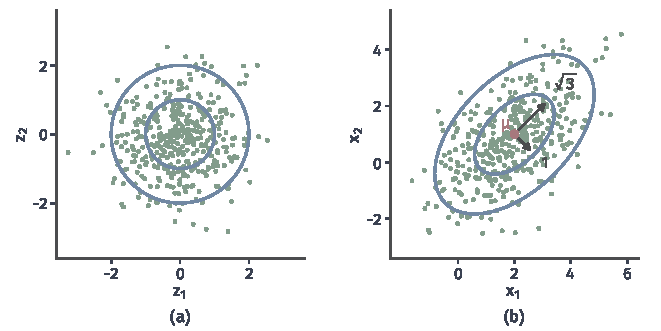
\includegraphics[width=112mm]{figures/07-probability/01-elementary-probability/matplotlib/mvd-gauss-affine/figure.pdf}
  \caption{仿射构造。(a)$400$个二维标准高斯点（绿，种子$7$）与半径$1$、$2$的圆（蓝）。(b)同一批点经$\bm{x}=\bm{\mu}+\bm{\Sigma}^{1/2}\bm{z}$映射后的位置，$\bm{\mu}=(2,1)^{\top}$（红点），$\Sigma_{1,1}=\Sigma_{2,2}=2$，$\Sigma_{1,2}=1$；圆变成椭圆，箭头是两条主轴方向，半轴长分别为$\sqrt3$与$1$。}
  \label{fig:mvd-gauss-affine}
\end{BookInlineFigure}

\paragraph{仿射变换与边缘分布}
构造方式本身就是仿射变换，所以再做一次仿射变换，结果仍是多元高斯。设$\bm{X}\sim\mathcal{N}(\bm{\mu},\bm{\Sigma})$，$\bm{M}$是$m\times d$矩阵，$\bm{c}\in\mathbb{R}^{m}$。把$\bm{X}$写成$\bm{\mu}+\bm{A}\bm{Z}$，
\[
 \bm{M}\bm{X}+\bm{c}=(\bm{M}\bm{\mu}+\bm{c})+(\bm{M}\bm{A})\bm{Z},\qquad (\bm{M}\bm{A})(\bm{M}\bm{A})^{\top}=\bm{M}\bm{\Sigma}\bm{M}^{\top} .
\]由定义~\ref{def:mvd-gaussian}，
\begin{equation}
 \bm{M}\bm{X}+\bm{c}\sim\mathcal{N}\bigl(\bm{M}\bm{\mu}+\bm{c},\ \bm{M}\bm{\Sigma}\bm{M}^{\top}\bigr) .
 \label{eq:mvd-gaussian-affine}
\end{equation}
这里不要求$\bm{M}$满秩，也不要求$m\leq d$。

两种特殊的$\bm{M}$最常用。取$\bm{M}$为单位矩阵的若干行，$\bm{M}\bm{X}$就是$\bm{X}$的一部分分量，于是边缘分布不必积分，只要从$\bm{\mu}$和$\bm{\Sigma}$中取出对应的子向量和子矩阵。取$\bm{M}=\bm{a}^{\top}$，得到一元线性组合
\[
 \bm{a}^{\top}\bm{X}\sim\mathcal{N}(\bm{a}^{\top}\bm{\mu},\ \bm{a}^{\top}\bm{\Sigma}\bm{a}) .
\]
方差为$0$时，$\mathcal{N}(m,0)$理解为恒取$m$的退化分布。

传感器例子中，$X_1\sim\mathcal{N}(2,2)$，$X_2\sim\mathcal{N}(1,2)$。两台读数之和与之差分别是
\[
 \begin{aligned}
  X_1+X_2&\sim\mathcal{N}(3,\,2+2+2\times1)=\mathcal{N}(3,6),\\
  X_1-X_2&\sim\mathcal{N}(1,\,2+2-2\times1)=\mathcal{N}(1,2) .
 \end{aligned}
\]
共享的扰动在和里叠加，在差里抵消，所以差的方差比和小。

\subsection{协方差与支撑}
\label{sec:mvd-gaussian-support}

定义~\ref{def:mvd-gaussian}只要求$\bm{\Sigma}$半正定。$\bm{\Sigma}$正定时，分布铺满整个$\mathbb{R}^{d}$，有普通的$d$维密度；$\bm{\Sigma}$奇异时，分布挤在一个低维的平面里。下面分别看这两种情形，再说明怎样判断一个随机向量是不是联合高斯。

\paragraph{正定协方差与密度}
$\bm{\Sigma}$正定时可以取方阵$\bm{A}$。例如Cholesky分解$\bm{\Sigma}=\bm{L}\bm{L}^{\top}$给出可逆的下三角矩阵$\bm{L}$（可参考\BookChapterRef{chap:direct-linear-solvers}{卷二第12章“线性方程的直接求解”}）。于是$\bm{X}=\bm{\mu}+\bm{L}\bm{Z}$是对标准高斯向量做可逆仿射变换，可以把$\bm{Z}$的密度搬过来。

\begin{theorem}[多元高斯密度]
\label{thm:mvd-gaussian-density}
设$\bm{\Sigma}$正定，$\bm{X}\sim\mathcal{N}(\bm{\mu},\bm{\Sigma})$，则$\bm{X}$有联合密度
\begin{equation}
 f_{\bm{X}}(\bm{x})=\frac{1}{(2\pi)^{d/2}(\det\bm{\Sigma})^{1/2}}\exp\Bigl(-\frac12Q(\bm{x})\Bigr),\qquad \bm{x}\in\mathbb{R}^{d},
 \label{eq:mvd-gaussian-density}
\end{equation}
其中
\begin{equation}
 Q(\bm{x})=(\bm{x}-\bm{\mu})^{\top}\bm{\Sigma}^{-1}(\bm{x}-\bm{\mu}) .
 \label{eq:mvd-gaussian-quadratic}
\end{equation}
\end{theorem}

\begin{proof}
对区域$S$，事件$\bm{X}\in S$就是$\bm{Z}\in\bm{L}^{-1}(S-\bm{\mu})$，所以
\[
 \mathbb{P}(\bm{X}\in S)=\int_{\bm{L}^{-1}(S-\bm{\mu})}\varphi_d(\bm{z})\,\mathrm{d}\bm{z} .
\]
作线性换元$\bm{z}=\bm{L}^{-1}(\bm{x}-\bm{\mu})$，积分区域变成$S$，体积元变为$\lvert\det\bm{L}^{-1}\rvert\,\mathrm{d}\bm{x}$。由$\det\bm{\Sigma}=(\det\bm{L})^{2}$，
\[
 \lvert\det\bm{L}^{-1}\rvert=(\det\bm{\Sigma})^{-1/2} .
\]
又$\bm{L}^{-\top}\bm{L}^{-1}=\bm{\Sigma}^{-1}$，所以$\lVert\bm{z}\rVert_2^{2}=Q(\bm{x})$。代入即得：$\bm{X}$落在$S$中的概率等于$f_{\bm{X}}$在$S$上的积分。
\end{proof}

公式的两部分各有来历。指数里的$Q(\bm{x})$是把偏离量$\bm{x}-\bm{\mu}$“还原”成标准高斯坐标后的平方长度；前面的$(\det\bm{\Sigma})^{-1/2}$是体积的缩放：$\bm{L}$把单位体积拉成$\det\bm{L}$倍，同样多的概率摊在更大的体积上，密度就按同一倍数降低。$d=1$时$Q=(x-\mu)^{2}/\sigma^{2}$，回到一元高斯密度。证明中的线性换元在第~\ref{chap:random-variable-transformations}章发展为一般的密度换元公式。

传感器例子中，$\det\bm{\Sigma}=3$，
\[
 \bm{\Sigma}^{-1}=\frac13\begin{bmatrix}2&-1\\-1&2\end{bmatrix} .
\]
记$u_1=x_1-2$，$u_2=x_2-1$，则$Q=\tfrac23(u_1^{2}-u_1u_2+u_2^{2})$，密度为
\[
 f_{\bm{X}}(\bm{x})=\frac{1}{2\sqrt3\,\pi}\exp\Bigl(-\frac{u_1^{2}-u_1u_2+u_2^{2}}{3}\Bigr) .
\]
在$\bm{x}=\bm{\mu}$处取最大值$1/(2\sqrt3\,\pi)\approx0.0919$。

\paragraph{等密度椭球与马氏距离}
密度只通过$Q(\bm{x})$依赖$\bm{x}$，等密度集是$Q(\bm{x})=c^{2}$。用谱分解
\[
 \bm{\Sigma}=\sum_{i=1}^{d}\lambda_i\bm{v}_i\bm{v}_i^{\top},\qquad \bm{\Sigma}^{-1}=\sum_{i=1}^{d}\lambda_i^{-1}\bm{v}_i\bm{v}_i^{\top},
\]
在以$\bm{\mu}$为原点、以$\bm{v}_i$为坐标轴的坐标$y_i=\bm{v}_i^{\top}(\bm{x}-\bm{\mu})$下，
\[
 Q(\bm{x})=\sum_{i=1}^{d}\frac{y_i^{2}}{\lambda_i} .
\]
所以$Q=c^{2}$是以$\bm{\mu}$为中心的椭球，主轴沿特征向量$\bm{v}_i$，半轴长为$c\sqrt{\lambda_i}$。方差大的方向椭球长，方差小的方向椭球扁。

量$\sqrt{Q(\bm{x})}$称为$\bm{x}$到$\bm{\mu}$的\term{马氏距离}（Mahalanobis distance）。它按各方向的波动大小度量偏离：沿方差大的方向走一段距离，算作较小的偏离。传感器例子的特征值是$3$和$1$，对应方向$(1,1)^{\top}/\sqrt2$与$(1,-1)^{\top}/\sqrt2$。两台读数同向偏离较常见，反向偏离较少见。

取两点$\bm{a}=\bm{\mu}+(1,1)^{\top}$和$\bm{b}=\bm{\mu}+(1,-1)^{\top}$，它们到$\bm{\mu}$的欧氏距离都是$\sqrt2$。代入$Q$，
\[
 Q(\bm{a})=\tfrac23(1-1+1)=\tfrac23,\qquad Q(\bm{b})=\tfrac23(1+1+1)=2 .
\]
两者相差$4/3$，密度之比为$\mathrm{e}^{2/3}\approx1.95$。图~\ref{fig:mvd-gauss-mahalanobis}(a)中，$\bm{a}$落在较内的椭圆上，$\bm{b}$落在较外的椭圆上，尽管两者在同一个欧氏圆上。

\begin{BookInlineFigure}
  \centering
  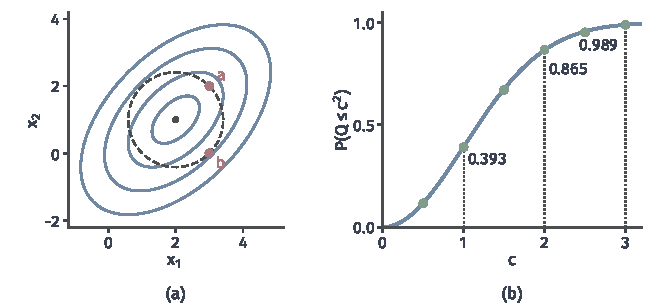
\includegraphics[width=112mm]{figures/07-probability/01-elementary-probability/matplotlib/mvd-gauss-mahalanobis/figure.pdf}
  \caption{马氏距离与椭圆概率。(a)传感器例子的等密度椭圆$Q=c^{2}$，$c=0.5,1,1.5,2$（蓝）；虚线圆是到$\bm{\mu}$（深灰点）欧氏距离为$\sqrt2$的点，红点$a$、$b$在圆上，马氏距离分别为$\sqrt{2/3}$与$\sqrt2$。(b)二维情形椭圆内的概率$1-\mathrm{e}^{-c^{2}/2}$（蓝），绿点是$4000$个模拟点（种子$11$）落入椭圆的比例。}
  \label{fig:mvd-gauss-mahalanobis}
\end{BookInlineFigure}

椭圆内的概率也可以直接算。$\bm{X}=\bm{\mu}+\bm{L}\bm{Z}$时，证明中已经看到$Q(\bm{X})=\lVert\bm{Z}\rVert_2^{2}$，所以$\mathbb{P}(Q(\bm{X})\leq c^{2})$与$\bm{\mu}$、$\bm{\Sigma}$都无关。$d=2$时用极坐标计算，
\[
 \mathbb{P}\bigl(\lVert\bm{Z}\rVert_2\leq c\bigr)=\int_0^{2\pi}\!\!\int_0^{c}\frac{1}{2\pi}\mathrm{e}^{-r^{2}/2}\,r\,\mathrm{d}r\,\mathrm{d}\theta=1-\mathrm{e}^{-c^{2}/2} .
\]
$c=1,2,3$时分别约为$0.393$、$0.865$、$0.989$。一元时均值加减一个标准差内有约$68\%$的概率，二维的“一个马氏距离”椭圆内只有约$39\%$：维数越高，概率越往外层分布。一般维数下$\lVert\bm{Z}\rVert_2^{2}$服从$\chi^2_d$分布，这在第~\ref{chap:random-variable-transformations}章说明。

\paragraph{奇异协方差与低维支撑}
现在设$\bm{\Sigma}$的秩$r<d$。定理~\ref{thm:mvd-gaussian-well-defined}的证明给出$\bm{X}$与$\bm{\mu}+\bm{B}\bm{W}$同分布，其中$\bm{B}$是$d\times r$矩阵，其列空间就是$\bm{\Sigma}$的列空间。$\bm{B}\bm{W}$总在这个列空间里，所以$\bm{X}$以概率$1$落在仿射子空间
\[
 \bm{\mu}+\{\bm{\Sigma}\bm{y}:\bm{y}\in\mathbb{R}^{d}\},
\]
其维数为$r$。这样的分布称为\term{退化高斯分布}（degenerate Gaussian distribution）。

退化的分布没有$d$维密度。$r<d$维的仿射子空间的$d$维体积为$0$，任何$d$维密度在它上面的积分都是$0$，不可能给它概率$1$。不过在子空间内部换用$r$个坐标$\bm{W}$，分布又是非退化的。

还可以从另一面看这件事。若$\bm{\Sigma}\bm{v}=\bm{0}$，则$\bm{v}^{\top}\bm{X}$的方差$\bm{v}^{\top}\bm{\Sigma}\bm{v}$为$0$，由式~\eqref{eq:mvd-gaussian-affine}，$\bm{v}^{\top}\bm{X}$服从$\mathcal{N}(\bm{v}^{\top}\bm{\mu},0)$，恒等于常数。零空间中的每个方向都对应$\bm{X}$满足的一条线性约束，$d-r$条约束把分布压进$r$维平面。

传感器例子中，令$S=X_1+X_2$，再记录$\bm{Y}=(S,2S)^{\top}$。取$\bm{M}$的两行分别为$(1,1)$和$(2,2)$，由式~\eqref{eq:mvd-gaussian-affine}，
\[
 \bm{Y}\sim\mathcal{N}\Biggl(\begin{bmatrix}3\\6\end{bmatrix},\ 6\begin{bmatrix}1&2\\2&4\end{bmatrix}\Biggr) .
\]
协方差矩阵的秩为$1$，零空间由$\bm{v}=(2,-1)^{\top}$张成，对应约束$2Y_1-Y_2=0$。图~\ref{fig:mvd-gauss-degenerate}(a)中所有样本点都在直线$y_2=2y_1$上；沿直线的坐标$S\sim\mathcal{N}(3,6)$有普通的一元密度，图~\ref{fig:mvd-gauss-degenerate}(b)。

\begin{BookInlineFigure}
  \centering
  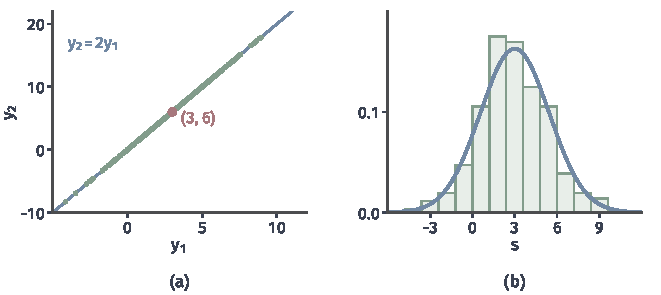
\includegraphics[width=112mm]{figures/07-probability/01-elementary-probability/matplotlib/mvd-gauss-degenerate/figure.pdf}
  \caption{退化高斯分布。(a)$\bm{Y}=(S,2S)^{\top}$的$300$个样本（绿，种子$5$），$S=X_1+X_2$；全部落在直线$y_2=2y_1$（蓝）上，红点为均值$(3,6)$。(b)沿直线的坐标$S$的直方图（浅绿）与$\mathcal{N}(3,6)$密度（蓝）。}
  \label{fig:mvd-gauss-degenerate}
\end{BookInlineFigure}

\paragraph{怎样判断联合高斯}
由式~\eqref{eq:mvd-gaussian-affine}，联合高斯向量的每个分量、每个线性组合$\bm{a}^{\top}\bm{X}$都服从一元高斯分布（方差可能为$0$）。反过来也成立：若对每个$\bm{a}\in\mathbb{R}^{d}$，$\bm{a}^{\top}\bm{X}$都服从一元高斯分布，则$\bm{X}$联合高斯。这个方向本章不证，证明要用到“特征函数唯一确定分布”，特征函数在第~\ref{chap:weak-convergence-of-distributions}章建立。它说明联合高斯是关于所有方向的条件，不是只关于坐标方向的条件。

只检查坐标方向是不够的。设$Z\sim\mathcal{N}(0,1)$，$S$以各$1/2$的概率取$\pm1$，与$Z$独立，考虑$(Z,SZ)$。第二个分量也服从$\mathcal{N}(0,1)$：
\[
 \mathbb{P}(SZ\leq t)=\tfrac12\mathbb{P}(Z\leq t)+\tfrac12\mathbb{P}(-Z\leq t)=\mathbb{P}(Z\leq t) ,
\]
这里用了$-Z$与$Z$同分布。两个分量都是标准高斯。

可是线性组合$Z+SZ$在$S=-1$时恒为$0$，所以$\mathbb{P}(Z+SZ=0)=1/2$。方差为正的一元高斯分布在单点上的概率为$0$，方差为$0$的又只取一个值，$Z+SZ$两样都不是，因而$(Z,SZ)$不是联合高斯。图~\ref{fig:mvd-random-sign}(a)中它的样本只落在两条对角线上，(b)中和的分布有一个质量为$1/2$的原子。

\begin{BookInlineFigure}
  \centering
  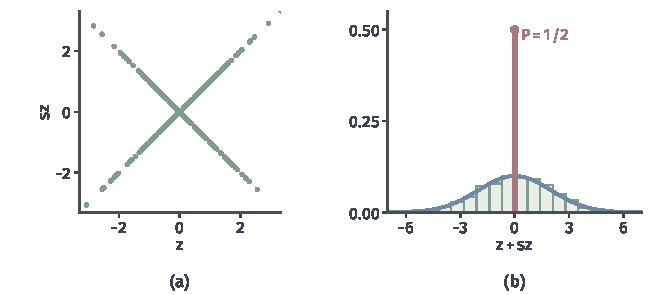
\includegraphics[width=112mm]{figures/07-probability/01-elementary-probability/matplotlib/mvd-random-sign/figure.pdf}
  \caption{分量各自高斯但不联合高斯。(a)$(Z,SZ)$的$400$个样本（绿，种子$3$），$S=\pm1$等可能且与$Z$独立；点只落在两条对角线上。(b)$Z+SZ$的分布：$0$处有概率$1/2$的原子（红），其余部分的密度为$\tfrac12$倍$\mathcal{N}(0,4)$密度（蓝），绿色直方图来自$4000$个模拟值。}
  \label{fig:mvd-random-sign}
\end{BookInlineFigure}

\subsection{条件分布与正交分解}
\label{sec:mvd-gaussian-conditional}

观测到第一台传感器的读数以后，第二台读数的分布变成什么？更一般地，把$\bm{X}$的分量分成两组，观测其中一组，另一组的条件分布是什么？两组什么时候相互独立？为此把$\bm{X}$与参数按相同方式分块：
\[
 \bm{X}=\begin{bmatrix}\bm{X}_a\\\bm{X}_b\end{bmatrix},\qquad
 \bm{\mu}=\begin{bmatrix}\bm{\mu}_a\\\bm{\mu}_b\end{bmatrix},\qquad
 \bm{\Sigma}=\begin{bmatrix}\bm{\Sigma}_{aa}&\bm{\Sigma}_{ab}\\\bm{\Sigma}_{ba}&\bm{\Sigma}_{bb}\end{bmatrix} ,
\]
其中交叉协方差$\bm{\Sigma}_{ab}$就是$\operatorname{Cov}(\bm{X}_a,\bm{X}_b)$，且$\bm{\Sigma}_{ba}=\bm{\Sigma}_{ab}^{\top}$。两组的边缘分布只用到对角块，两组之间的联系全部记在$\bm{\Sigma}_{ab}$里。

\paragraph{零交叉协方差推出独立}
第~\ref{chap:random-vectors}章说明，独立推出不相关，反过来一般不成立。联合高斯是一个重要的例外。

\begin{theorem}[联合高斯的分块独立]
\label{thm:mvd-gaussian-independence}
设$\bm{X}\sim\mathcal{N}(\bm{\mu},\bm{\Sigma})$按上述方式分块。若$\bm{\Sigma}_{ab}=\bm{0}$，则$\bm{X}_a$与$\bm{X}_b$相互独立。
\end{theorem}

\begin{proof}
取矩阵$\bm{A}_a$、$\bm{A}_b$使$\bm{A}_a\bm{A}_a^{\top}=\bm{\Sigma}_{aa}$，$\bm{A}_b\bm{A}_b^{\top}=\bm{\Sigma}_{bb}$，列数分别为$k_a$、$k_b$，再令
\[
 \bm{A}=\begin{bmatrix}\bm{A}_a&\bm{0}\\\bm{0}&\bm{A}_b\end{bmatrix} .
\]
因为$\bm{\Sigma}_{ab}=\bm{0}$，有$\bm{A}\bm{A}^{\top}=\bm{\Sigma}$。由定理~\ref{thm:mvd-gaussian-well-defined}，$\bm{X}$与$\bm{\mu}+\bm{A}\bm{Z}$同分布。把$\bm{Z}$分成前$k_a$个分量$\bm{Z}'$与后$k_b$个分量$\bm{Z}''$，就有
\[
 \bm{X}_a\overset{\mathrm{d}}{=}\bm{\mu}_a+\bm{A}_a\bm{Z}',\qquad \bm{X}_b\overset{\mathrm{d}}{=}\bm{\mu}_b+\bm{A}_b\bm{Z}'' ,
\]
这里$\overset{\mathrm{d}}{=}$表示两组同时同分布。

$\bm{Z}'$与$\bm{Z}''$由不同的独立分量组成，联合密度是两部分密度之积，因而相互独立。对区域$S$、$T$，记$S'$、$T''$为它们在两个仿射映射下的原像，于是
\[
 \mathbb{P}(\bm{X}_a\in S,\ \bm{X}_b\in T)=\mathbb{P}(\bm{Z}'\in S',\ \bm{Z}''\in T'')=\mathbb{P}(\bm{Z}'\in S')\,\mathbb{P}(\bm{Z}''\in T'') .
\]
右边两个因子分别是$\mathbb{P}(\bm{X}_a\in S)$与$\mathbb{P}(\bm{X}_b\in T)$。
\end{proof}

证明没有用到密度，所以$\bm{\Sigma}$奇异时同样成立。逐个分量应用：联合高斯向量的协方差矩阵若是对角的，各分量相互独立。

定理的前提是整个向量联合高斯。上一小节的$(Z,SZ)$中，
\[
 \operatorname{Cov}(Z,SZ)=\mathbb{E}[S]\,\mathbb{E}[Z^{2}]=0 ,
\]
两个分量不相关，也都是标准高斯，却不独立：$\lvert SZ\rvert=\lvert Z\rvert$，知道$Z$以后，$SZ$只剩$\pm Z$两种可能。定理不适用，正是因为它们不联合高斯。

\paragraph{配方求条件分布}
设$\bm{\Sigma}$正定，于是对角块$\bm{\Sigma}_{bb}$也正定，可逆。目标是把联合密度写成“$\bm{x}_b$的边缘密度”乘以“$\bm{x}_a$的某个高斯密度”。关键是对二次型$Q$关于$\bm{x}_a$配方，用矩阵语言就是一步分块消元。令
\[
 \bm{K}=\bm{\Sigma}_{ab}\bm{\Sigma}_{bb}^{-1},\qquad
 \bm{S}=\bm{\Sigma}_{aa}-\bm{\Sigma}_{ab}\bm{\Sigma}_{bb}^{-1}\bm{\Sigma}_{ba},\qquad
 \bm{E}=\begin{bmatrix}\bm{I}&-\bm{K}\\\bm{0}&\bm{I}\end{bmatrix} .
\]
$\bm{S}$是$\bm{\Sigma}$中块$\bm{\Sigma}_{bb}$的Schur补（可参考\BookChapterRef{chap:direct-linear-solvers}{卷二第12章“线性方程的直接求解”}）。

先左乘$\bm{E}$。第一块行的第二块变为$\bm{\Sigma}_{ab}-\bm{K}\bm{\Sigma}_{bb}=\bm{0}$，
\[
 \bm{E}\bm{\Sigma}=\begin{bmatrix}\bm{S}&\bm{0}\\\bm{\Sigma}_{ba}&\bm{\Sigma}_{bb}\end{bmatrix} .
\]
再右乘$\bm{E}^{\top}$。第二块行的第一块变为$\bm{\Sigma}_{ba}-\bm{\Sigma}_{bb}\bm{K}^{\top}$，由$\bm{\Sigma}_{bb}\bm{K}^{\top}=\bm{\Sigma}_{ba}$，它也是$\bm{0}$，得到
\begin{equation}
 \bm{E}\bm{\Sigma}\bm{E}^{\top}=\begin{bmatrix}\bm{S}&\bm{0}\\\bm{0}&\bm{\Sigma}_{bb}\end{bmatrix} .
 \label{eq:mvd-block-elimination}
\end{equation}

式~\eqref{eq:mvd-block-elimination}给出三件事。$\bm{E}$可逆，所以右边与$\bm{\Sigma}$同为正定，$\bm{S}$正定。$\det\bm{E}=1$，所以行列式按块分解。两边求逆，又得到$\bm{\Sigma}^{-1}$的分解：
\[
 \det\bm{\Sigma}=\det\bm{S}\cdot\det\bm{\Sigma}_{bb},\qquad
 \bm{\Sigma}^{-1}=\bm{E}^{\top}\begin{bmatrix}\bm{S}^{-1}&\bm{0}\\\bm{0}&\bm{\Sigma}_{bb}^{-1}\end{bmatrix}\bm{E} .
\]

把最后一式代入$Q$。记$\bm{u}=\bm{x}-\bm{\mu}$，则$\bm{E}\bm{u}$的两块是$\bm{u}_a-\bm{K}\bm{u}_b$与$\bm{u}_b$，于是
\[
 Q(\bm{x})=(\bm{u}_a-\bm{K}\bm{u}_b)^{\top}\bm{S}^{-1}(\bm{u}_a-\bm{K}\bm{u}_b)+\bm{u}_b^{\top}\bm{\Sigma}_{bb}^{-1}\bm{u}_b .
\]
这就是配方的结果：第一项是$\bm{x}_a$围绕$\bm{\mu}_a+\bm{K}\bm{u}_b$的二次型，第二项只含$\bm{x}_b$。

把配方结果和行列式的分解代入式~\eqref{eq:mvd-gaussian-density}，常数与指数都按两组拆开，联合密度成为两个高斯密度之积：第一个是$\bm{x}_a$的均值为$\bm{\mu}_a+\bm{K}\bm{u}_b$、协方差为$\bm{S}$的密度，第二个是$\mathcal{N}(\bm{\mu}_b,\bm{\Sigma}_{bb})$的密度。后者正是$\bm{X}_b$的边缘密度。除以它，按第~\ref{chap:random-vectors}章条件密度的定义得到下面的定理。

\begin{theorem}[高斯条件分布]
\label{thm:mvd-gaussian-conditional}
设$\bm{\Sigma}$正定，$\bm{X}\sim\mathcal{N}(\bm{\mu},\bm{\Sigma})$按上述方式分块。对每个$\bm{x}_b$，给定$\bm{X}_b=\bm{x}_b$时$\bm{X}_a$的条件分布是高斯分布，条件均值与条件协方差分别为
\begin{align}
 \mathbb{E}[\bm{X}_a\mid\bm{X}_b=\bm{x}_b]&=\bm{\mu}_a+\bm{\Sigma}_{ab}\bm{\Sigma}_{bb}^{-1}(\bm{x}_b-\bm{\mu}_b),
 \label{eq:mvd-gauss-cond-mean}\\
 \operatorname{Cov}(\bm{X}_a\mid\bm{X}_b=\bm{x}_b)&=\bm{\Sigma}_{aa}-\bm{\Sigma}_{ab}\bm{\Sigma}_{bb}^{-1}\bm{\Sigma}_{ba} .
 \label{eq:mvd-gauss-cond-cov}
\end{align}
\end{theorem}

回到传感器，观测第一台读数$X_1=x_1$，求第二台$X_2$的条件分布。此时$\bm{X}_a=X_2$，$\bm{X}_b=X_1$，各块都是数：$\Sigma_{aa}=\Sigma_{bb}=2$，$\Sigma_{ab}=1$。代入式~\eqref{eq:mvd-gauss-cond-mean}和式~\eqref{eq:mvd-gauss-cond-cov}，
\[
 \mathbb{E}[X_2\mid X_1=x_1]=1+\frac{x_1-2}{2},\qquad \operatorname{Var}(X_2\mid X_1=x_1)=2-\frac{1}{2}=\frac32 .
\]

若第一台读到$x_1=4$，比均值高$2$，则$X_2\mid X_1=4\sim\mathcal{N}(2,3/2)$。观测之前$X_2\sim\mathcal{N}(1,2)$，$\mathbb{P}(X_2>2)=1-\Phi(1/\sqrt2)\approx0.240$，其中$\Phi$是标准高斯分布函数；观测之后，$\mathbb{P}(X_2>2\mid X_1=4)=0.5$。第一台偏高，把对第二台的预测中心从$1$推到$2$，方差从$2$缩到$1.5$。

图~\ref{fig:mvd-gauss-conditional}(a)中，竖直红线$x_1=4$切过等密度椭圆，切片上的密度重新归一化，就是条件密度；黄线是条件均值$m(x_1)=1+(x_1-2)/2$，它穿过每条竖直切片上密度最高的点。(b)比较了观测前后$X_2$的密度。

\begin{BookInlineFigure}
  \centering
  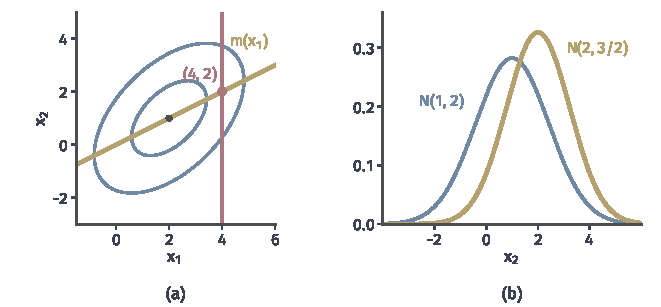
\includegraphics[width=112mm]{figures/07-probability/01-elementary-probability/matplotlib/mvd-gauss-conditional/figure.pdf}
  \caption{传感器例子的条件化。(a)等密度椭圆$Q=1,4$（蓝），观测$x_1=4$（红线），条件均值直线$m(x_1)=1+(x_1-2)/2$（黄），红点$(4,2)$是给定$X_1=4$时$X_2$的条件均值。(b)$X_2$的边缘密度$\mathcal{N}(1,2)$（蓝）与给定$X_1=4$后的条件密度$\mathcal{N}(2,3/2)$（黄）。}
  \label{fig:mvd-gauss-conditional}
\end{BookInlineFigure}

式~\eqref{eq:mvd-gauss-cond-mean}与式~\eqref{eq:mvd-gauss-cond-cov}有两个特点。条件均值是观测值的仿射函数，图中是一条直线。条件协方差完全不依赖观测值：无论第一台读到多少，第二台的剩余不确定性都是$1.5$。一般的联合分布中，条件方差会随条件取值变化，例如三角形区域上的均匀分布，固定的坐标越靠近顶点，另一个坐标可取的范围越窄，条件方差越小。不随观测值变化是高斯模型的特殊性质。

此外，$\bm{\Sigma}_{aa}$与$\bm{S}$之差是半正定矩阵$\bm{\Sigma}_{ab}\bm{\Sigma}_{bb}^{-1}\bm{\Sigma}_{ba}$，所以观测只会减少每个方向上的方差，不会增加。$\bm{\Sigma}_{ab}=\bm{0}$时$\bm{S}=\bm{\Sigma}_{aa}$，条件分布等于边缘分布，与定理~\ref{thm:mvd-gaussian-independence}一致。

\paragraph{正交分解}
条件协方差为什么不随观测值变化？把$\bm{X}_a$减去它的条件均值，看剩下的残差
\[
 \bm{R}=\bm{X}_a-\bm{\mu}_a-\bm{K}(\bm{X}_b-\bm{\mu}_b) .
\]
$(\bm{R},\bm{X}_b)$是$\bm{X}$的仿射像，由式~\eqref{eq:mvd-gaussian-affine}联合高斯。它们的交叉协方差是
\[
 \operatorname{Cov}(\bm{R},\bm{X}_b)=\bm{\Sigma}_{ab}-\bm{K}\bm{\Sigma}_{bb}=\bm{0} .
\]
由定理~\ref{thm:mvd-gaussian-independence}，$\bm{R}$与$\bm{X}_b$独立。

再算残差的协方差。展开后有三项交叉项，每一项都等于$\bm{\Sigma}_{ab}\bm{\Sigma}_{bb}^{-1}\bm{\Sigma}_{ba}$，于是
\[
 \operatorname{Cov}(\bm{R})=\bm{\Sigma}_{aa}-\bm{K}\bm{\Sigma}_{ba}-\bm{\Sigma}_{ab}\bm{K}^{\top}+\bm{K}\bm{\Sigma}_{bb}\bm{K}^{\top}=\bm{S} .
\]
所以$\bm{X}_a$分解成两部分：
\begin{equation}
 \bm{X}_a=\underbrace{\bm{\mu}_a+\bm{K}(\bm{X}_b-\bm{\mu}_b)}_{\text{由}\bm{X}_b\text{决定}}+\underbrace{\bm{R}}_{\text{与}\bm{X}_b\text{独立}},\qquad \bm{R}\sim\mathcal{N}(\bm{0},\bm{S}) .
 \label{eq:mvd-orthogonal-decomposition}
\end{equation}

观测$\bm{X}_b=\bm{x}_b$只确定了第一部分，残差的分布不受影响，所以条件分布是把$\mathcal{N}(\bm{0},\bm{S})$平移到条件均值处。$\bm{K}$的选择恰好使残差与$\bm{X}_b$不相关；用协方差作内积，第一部分就是$\bm{X}_a$在“$\bm{X}_b$的仿射函数”上的正交投影。对联合高斯，不相关又等于独立，于是投影之外不再剩下任何与$\bm{X}_b$有关的东西。

传感器例子中，$X_2$的残差是
\[
 R=X_2-1-\frac{X_1-2}{2}=-\frac12Z_1+\frac12Z_2+Z_3 .
\]
它与$X_1=2+Z_1+Z_2$的协方差是$-\tfrac12+\tfrac12=0$：$Z_1$与$Z_2$的贡献恰好抵消。方差为$\tfrac14+\tfrac14+1=\tfrac32$，与式~\eqref{eq:mvd-gauss-cond-cov}一致。

正交分解的论证只用到$\bm{\Sigma}_{bb}$可逆，不需要整个$\bm{\Sigma}$正定。$\bm{S}$奇异时$\bm{X}$没有联合密度，第~\ref{chap:random-vectors}章的密度比无法直接使用，但式~\eqref{eq:mvd-orthogonal-decomposition}仍说明，给定$\bm{X}_b=\bm{x}_b$后$\bm{X}_a$应当服从$\mathcal{N}(\bm{\mu}_a+\bm{K}(\bm{x}_b-\bm{\mu}_b),\bm{S})$，这是一个退化高斯分布。对零概率条件的严格表述在第~\ref{chap:conditional-distributions}章给出。

\paragraph{观测块退化}
若$\bm{\Sigma}_{bb}$也奇异，观测的各分量之间有线性约束，观测值只能落在$\bm{\mu}_b$加上$\bm{\Sigma}_{bb}$列空间的仿射子空间里，此外的观测值不可能出现。例如增加第三台传感器，它只是第一台的复制品，$X_3=X_1$。观测$(X_1,X_3)=(4,4)$与只观测$X_1=4$含有相同的信息，而$(4,5)$根本不会出现。处理办法是先限制到有效支撑：去掉冗余的分量，只对一组线性无关的观测条件化。

不挑选分量也可以，把$\bm{\Sigma}_{bb}^{-1}$换成Moore--Penrose伪逆$\bm{\Sigma}_{bb}^{+}$（可参考\BookChapterRef{chap:linear-solution-selection}{卷二第11章“线性方程与最小二乘的选解”}），令$\bm{K}=\bm{\Sigma}_{ab}\bm{\Sigma}_{bb}^{+}$。正交分解仍然成立，只需验证$\bm{K}\bm{\Sigma}_{bb}=\bm{\Sigma}_{ab}$。

验证分两步。若$\bm{\Sigma}_{bb}\bm{v}=\bm{0}$，则$\bm{v}^{\top}\bm{X}_b$方差为$0$，恒为常数，它与$\bm{X}_a$的协方差$\bm{\Sigma}_{ab}\bm{v}$为$\bm{0}$；所以$\bm{\Sigma}_{bb}$的零空间含于$\bm{\Sigma}_{ab}$的零空间。又$\bm{I}-\bm{\Sigma}_{bb}^{+}\bm{\Sigma}_{bb}$是到$\bm{\Sigma}_{bb}$零空间的正交投影，于是
\[
 \bm{\Sigma}_{ab}-\bm{K}\bm{\Sigma}_{bb}=\bm{\Sigma}_{ab}\bigl(\bm{I}-\bm{\Sigma}_{bb}^{+}\bm{\Sigma}_{bb}\bigr)=\bm{0} .
\]
此后的论证与前面相同。

\paragraph{样本平均与残差}
正交分解在高斯样本上有一个重要推论。设$X_1,\ldots,X_n$独立同分布于$\mathcal{N}(\mu,\sigma^{2})$，$\sigma>0$，排成向量$\bm{X}=\mu\bm{1}+\sigma\bm{Z}$，于是$\bm{X}\sim\mathcal{N}(\mu\bm{1},\sigma^{2}\bm{I}_n)$。考虑样本平均与残差向量
\[
 \bar{X}_n=\frac1n\bm{1}^{\top}\bm{X},\qquad \bm{R}=\bm{X}-\bar{X}_n\bm{1}=\bm{P}\bm{X},\qquad \bm{P}=\bm{I}_n-\frac1n\bm{1}\bm{1}^{\top} .
\]

几何上，$\bar{X}_n\bm{1}$是$\bm{X}$在直线$\{c\bm{1}\}$上的正交投影，$\bm{R}$是垂直于这条直线的部分。例如观测值$\bm{x}=(1,2,6)^{\top}$，平均为$3$，
\[
 \bm{x}=(3,3,3)^{\top}+(-2,-1,3)^{\top},
\]
第二个向量各分量之和为$0$，与$\bm{1}$正交，图~\ref{fig:mvd-mean-residual}。

\begin{BookInlineFigure}
  \centering
  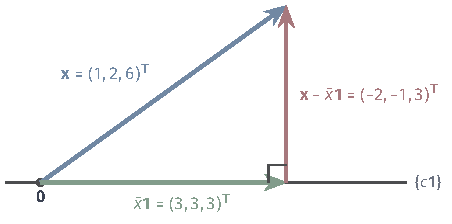
\includegraphics[width=77mm]{figures/07-probability/01-elementary-probability/tikz/mvd-mean-residual/figure.pdf}
  \caption{观测向量$\bm{x}=(1,2,6)^{\top}$（蓝）的正交分解，画在$\bm{1}$与$\bm{x}$张成的平面内并按比例绘制。绿色箭头是在直线$\{c\bm{1}\}$上的投影$\bar{x}\bm{1}$，红色箭头是残差$\bm{x}-\bar{x}\bm{1}$，两者垂直。}
  \label{fig:mvd-mean-residual}
\end{BookInlineFigure}

$(\bar{X}_n,\bm{R})$是$\bm{X}$的线性像，联合高斯。交叉协方差为
\[
 \operatorname{Cov}(\bm{R},\bar{X}_n)=\bm{P}\,(\sigma^{2}\bm{I}_n)\,\frac1n\bm{1}=\frac{\sigma^{2}}{n}\bm{P}\bm{1}=\bm{0} ,
\]
因为$\bm{P}\bm{1}=\bm{1}-\bm{1}=\bm{0}$。由定理~\ref{thm:mvd-gaussian-independence}，$\bar{X}_n$与整个残差向量独立，因而与残差平方和$\lVert\bm{R}\rVert_2^{2}$独立。

两部分的分布也能读出来。$\bar{X}_n\sim\mathcal{N}(\mu,\sigma^{2}/n)$。$\bm{R}\sim\mathcal{N}(\bm{0},\sigma^{2}\bm{P})$，$\bm{P}$是到$n-1$维子空间的正交投影，秩为$n-1$，所以$\bm{R}$是一个退化高斯向量，只在分量和为$0$的超平面上取值。

残差平方和的分布可以用旋转不变性求出。取正交矩阵$\bm{Q}$，其第一行为$\bm{1}^{\top}/\sqrt n$，令$\bm{Y}=\bm{Q}\bm{Z}$，由引理~\ref{lem:mvd-rotation}它仍是标准高斯向量，且$Y_1=\sqrt n\,\bar{Z}$，$\lVert\bm{Y}\rVert_2=\lVert\bm{Z}\rVert_2$。于是
\[
 \sum_{i=1}^{n}(Z_i-\bar{Z})^{2}=\lVert\bm{Z}\rVert_2^{2}-n\bar{Z}^{2}=\sum_{i=2}^{n}Y_i^{2} .
\]
右边是$n-1$个独立标准高斯变量的平方和，服从$\chi^2_{n-1}$（第~\ref{chap:random-variable-transformations}章），所以$\sum_i(X_i-\bar{X}_n)^{2}/\sigma^{2}\sim\chi^2_{n-1}$。样本平均与样本方差独立，是高斯模型统计推断的出发点，可参考\BookChapterRef{chap:parametric-statistical-inference}{卷八第1章“参数化统计推断”}。

这个独立性依赖联合高斯，不是样本平均与残差的一般性质。对任何有限方差的独立同分布样本，$\operatorname{Cov}(\bm{R},\bar{X}_n)=\bm{0}$都成立，但不相关推不出独立。图~\ref{fig:mvd-mean-variance}对比两种总体：高斯样本的平均与残差平方和看不出关系，指数样本的平均越大，残差平方和越分散。

\begin{BookInlineFigure}
  \centering
  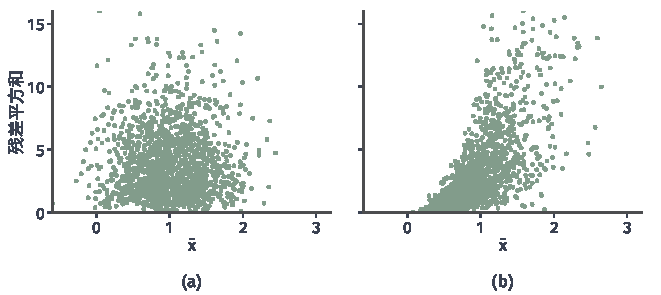
\includegraphics[width=112mm]{figures/07-probability/01-elementary-probability/matplotlib/mvd-mean-variance/figure.pdf}
  \caption{样本平均与残差平方和，每组$n=5$个观测，重复$1500$组。(a)$\mathcal{N}(1,1)$样本（种子$21$），两者的样本相关系数约为$0.02$。(b)$\operatorname{Exp}(1)$样本（均值与方差同为$1$，种子$22$），样本相关系数约为$0.68$，平均越大残差平方和越大。}
  \label{fig:mvd-mean-variance}
\end{BookInlineFigure}
